\documentclass{proseminar}

\let\i\undefined
\let\c\undefined
\let\b\undefined
\newcommand{\i}[1]{\emph{#1}}
\newcommand{\c}[1]{\texttt{#1}}
\newcommand{\b}[1]{\textbf{#1}}
\begin{document}

\conferenceinfo{Albert-Ludwigs Universit\"at Freiburg\\Technische Fakult\"at, Institut f\"ur Informatik\\Lehrstuhl f\"ur Datenbanken \& Informationssysteme}{}

\title{Trust and Privacy in Social Media \\
\huge Content oriented trust}

\numberofauthors{1} 
\author{
Tim Schmiedl\\
\email{tim.schmiedl@neptun.uni-freiburg.de}
}

\maketitle

\section{Introduction}
Over the last couple of years microblogging became a well-established paradigm for interaction in online social networks.
Especially the success of Twitter let to an increase of huge amount of real-time informations on the internet. It lets user post short messages which are shown immeadietly for their followers. This concept was of course quickly adapted by news agencies, product pages and many other. So nowadays Twitter displays a wide variety of content. Most tweets correspond to the following categories; conversation items, wich are just valuable to user and its immediate circle of friends, or infomation or news items, which could be interesting for a broader community.

%* mobile internet devices 
%* propagating news and information about developing events 

% =========================

\subsection*{Current Situation}
Twitter was well known to display tweets in reverse cronical order displaying what is happening right now on the very top of the news feed. 
The microblogging company itself tried to experiement in some ways to show the information in different ways, one is to show popular tweets on top regardless of the posting time.
This decision was often critized as it often shows for the user unrelevant information or advertisment. This position of popular tweet was also often the target of internet trolls or spammers trying polute the news feed of many users.

As microblogging has become more and more popular it was shown that beside chatting about events on a day-to-day basis it can be in particularly helpful during emergency and/or crisis situations.
Twitter provide real-time information from the actual location where the crisis is unfolding. This information often spreads faster and to a wider audience than what traditional news media sources can achieve.


% =========================

\subsection*{Problems}
Twitters ranking method of displaying popular tweets as not taken into account content relevance or the twitter account.
This lets a large amount of pointless tweets may flood the relevant tweets of the users news feed. It also allows for more potential for spam to spead, as it is not filtered in this ranking method.

As a result of the big variety of content and different kinds of users it is very difficult to differenciate between news related topics and chat between user. Finding tweets which have valuable information outside its immediate circle of friends or follower is often not easy as there is no distinction between different kind of messages. 


% =========================

\subsection*{Goals of the Papers}
The primary element of this report are the two papers...

In P2 they propose a method to rank tweets based on their content relevance to a given query. They use different set of features to find out weather a tweet is interesting for a user. Their \i{learning to rank} algorithm considers content relevance as well as account authority and twitter-specific features to rank tweets. In their evaluation they find out that especially if a URL is present in the tweet improves the relevance as well as that just the number of followers to an account doesn't directly correlates to bigger relevances of tweets from that author.

In P1 the authors had a the main focus on the credibility of time-sensitive information, in particular on current news events. In a previous step they also try to automatically assess the newsworthiness of a discussion topic. This is to differenciate between the chatter and news related messages circulating on twitter in unsorted way. Both newsworthiness and credibility play an equally important role in this paper.

% =========================
% =========================
% =========================


\section{Twitter Case Study}
* from P1: Predicting information credibility in time-sensitive social media

* earthquake that hit Chile on February 2010

* Event characterization

* Twitter reaction: Information propagation behavior \& False rumor propagation


% =========================
% =========================
% =========================

\section{Proposed Method: Ranking of \\Tweets}
This section describes the method of ranking of tweets introduced in P2. 
Their \textit{learning to Rank} method is a data-driven approach to assign a score to tweet. 
For training the ranking model the RankSVM alogrith is used.

Figure \ref{fig:p2overview} shows the the paradigm of the method and the separation of the trainign and test corpus.

\begin{figure}[h]
\centering
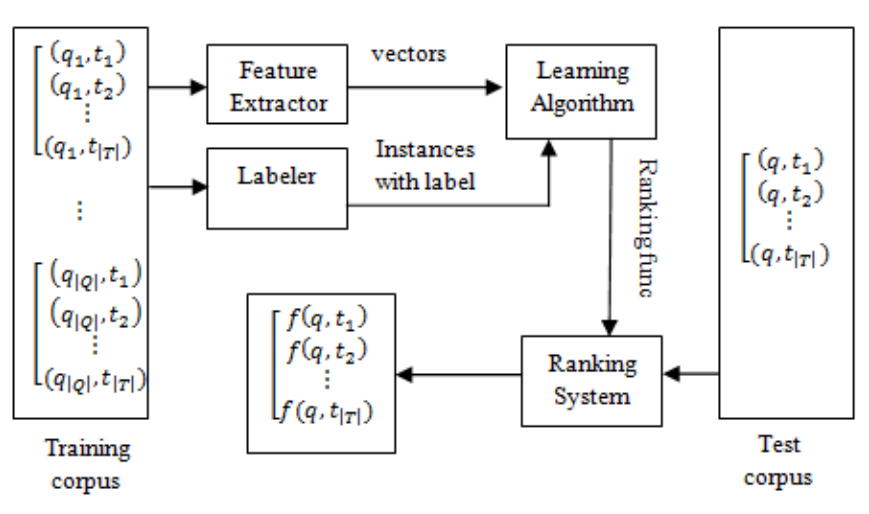
\epsfig{file=img/p2_overview.png, width=0.45\textwidth}
\caption{General Paradigm of Learning for Tweets Ranking}
\label{fig:p2overview}
\end{figure}

The learning to rank system used three types of featrues: Content relevance features, Twitter specific features and Account authority features

\subsubsection*{Content relevance features}
The content relevance features refer to those features which describe the content relevance between queries and tweets.
P1 uses three different types of content relavance:

\begin{itemize}
\item \b{Okapi BM25} score measures the relavance between query and tweet. It considers the length of a tweet, the average length of tweets and the Inverse Document Frequency.
\item \b{Similarity of contents} how many tweets of the query are similar in content with the current tweet. To accomplish that the cosine similarity between every pair of tweets is computed.
\item \b{Length} is simply measured by the number of words that a tweet contains.
\end{itemize}


\subsubsection*{Twitter Specific Features}
As the proposed method is tested on twitter it also relys on some of the Tweet-specific features. 

\begin{itemize}
\item \b{URL and URL Count} Tweets can contains one ore more URLs in the composed message. The feature URL hereby is a binary feature indicating with 1 if there is a URL present, whereas the URL Count extimates how often a particular URL is found in the tweet corpus.
\item \b{Retweet Count} Twitter users can forward a tweet to his or her followers with or without modification on the forwarded tweets. In this feature Retweet count is defined as the number of times a tweet is retweeted.
\item \b{Hash Tag Score} Hashtags are a type of label or metadata tag microblogging services, especially on twitter, which makes it easier for users to find messages with a specific theme or content. For this feature hashtags are collected from all tweets and sorted in descending order. The feature score correlates with the frequency of hashtags in the tweet with the most frequent hashtags.
\item \b{Reply} This is a binary feature. It is 1 when the tweet is a reply and 0 otherwise.
\item \b{Words out of vocabulary} This feature is used to roughly approximate the language quality of tweets. The vocabulary is defined by the words of a dictionary with 0.5 million entries.

\end{itemize}

\subsubsection*{Account Authority Features}
+ There are three important relations between users in Twitter: follow, retweet, and mention. 

+ user are more authoritative: more followers, been mentioned in more tweets, listed in more lists and retweeted by more important users

+ tweet is more likly to be informative if posted or retweeted by authoritative user

+ Scores: Follower, Mention, List, Popularity (computed by PageRank)

% =========================
% =========================
% =========================

\section{Proposed Method: Prediction\\ Model for Tweets}
* method of P1: Predicting information credibility in time-sensitive social media

* The main focus credibility of time-sensitive information, in particular on current news events. 

* newsworthiness of a discussion topic, and that of determining its credibility, are equally important


\subsection{Retrieving and Labeling of Data}
* information cascade, which is composed of all of the messages which usually accompany newsworthy events

* detected by Twitter Monitor (keyword-based query), detection of events see Mathioudakis and Koudas, 2010

* 2 month monitoring, keep topics with at most 10.000 tweets = 2.500 topics w 1,873,000 messages (initial topic data)


\subsubsection*{Newsworthyness}
* first step seperate newsworthy topics vs conversation/chat etc.: manual data labeleling procress, Crowdsourcing with Mechanical Turk

* human editor label Data as: NEWS / Chat / Unsure

* short summary sentence for the topic, reduce the effect of click spammers

* Result: 35.6 (136 cases) UNSURE, 29.5 percent NEWS (113 cases), 34.9 percent CHAT (134 cases).

\subsubsection*{Credibility}
* second round: newsworthy topics should be rated in credibility

* input is the output of the automatic classifier based on the data extracted in the first step

* 747 topics with NEWS label presented to human evaluator for judgement

* 4 different credibility classes: "almost certainly true" (306 cases), "likely to be false" 31.8 percent (237 cases), "almost certainly false" 8.6
percent (65 cases), 18.6 percent (139 cases) uncertain.

\subsection{Prediction Model for Tweets}
* main hypothesis is that the level of newsworthiness and credibility can be estimated automatically.

\subsubsection*{Automatic discovery of newsworthy topics}
* labeled data as training set for different learning schemes. Bayes Net best for the scenario (Random forest comparable results)

* different factors show credible:

* 1. reactions and emotion, opions, negative/positive sentiments 

* 2. certainty, question info or not?

* 3. sources cited, URLs, popular domain

* 4. propagation characteristics, which user, how many follower etc.

* Feature subsets: Text-only, User subset, Topic subset, Propagation subset

* Text: length of tweet, sentiment-based features, URLs, Twitter-specific: hashtags, user mentions (20 features)

* User: aggregated properties of authors like \#friends \#followers (7 features)

* Topic: most frequent URL, most frequent hashtag, most frequent user mention, and most frequent author (4 features)

* the propagation-based features, fraction of re-tweets, total number of tweets (7 features)

\begin{figure}[h]
\centering
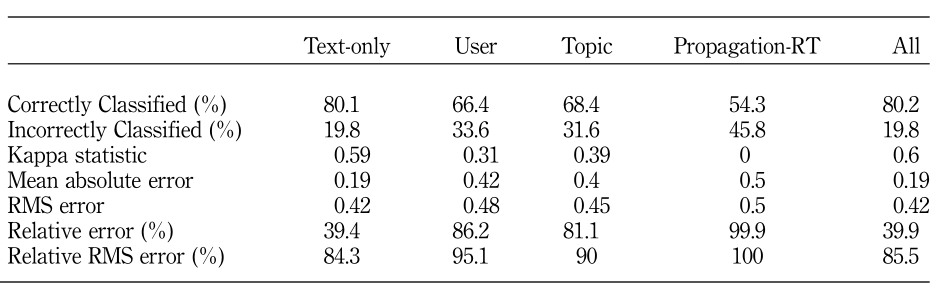
\epsfig{file=img/p1_table_feature_subset.png, width=0.45\textwidth}
\caption{Results for different feature subsets}
\end{figure}

\subsubsection*{Credibility prediction}
* how to automatically assign a credibility level (or score) to a topic deemed newsworthy by our previous classifier

* binary classification: CREDIBLE , NOT-CREDIBLE 47.2/52.8 percent. In total, these topics involve 165,312 tweets

* study how different learning algorithms perform in particular learning scenario

* predictability of the problem is very difficult, with very moderated k-statistic values (see Evaluation)

* Feature selection: evaluate 684 subsets, best results with 16 features

* fraction of tweets having a positive/negative sentiment; 

* fraction of tweets with URL, URL top 10.000 urls

* tweets containing: question mark, exclamation mark, first- /second-person pronoun, emoticons

% =========================
% =========================
% =========================

\section{Evaluation}
\subsection{Predicting information credibility in time-sensitive social media}

\subsubsection*{Credibility}
* predictability of the problem is very difficult, with very moderated k-statistic values

* main conclusions are that misclassification of not-credible topics as credible is significant, but recall rates are quite acceptable.

* features positive for credibility: more friends, more URLs + urls in popular 10.000, longer in general, negative sentiments

* features negative for credibility: positive polarity, more question and exclamation marks, first and third-persion pronouns

% =========================

\subsection{An Empirical Study on Learning to Rank of Tweets}
\subsubsection*{Dataset}
+ 20 query terms on CrowdEye (5 persons, 5 locations, 5 products and 5 movie names)

+ 159,298 tweets

+ 500 tweets/topic evaluated by human editor: labeled with grade 4 judgements 

+ Excellent 20.9 \% ; Good 10.9\%; Fair 16.9\%; Bad 51.3\% 

\subsubsection*{Results}
+ different methods tested in Five-fold cross-validation of tweets in 16 queries: chronological order, account authority, and content relevance + combinded
\begin{figure}[h]
\centering
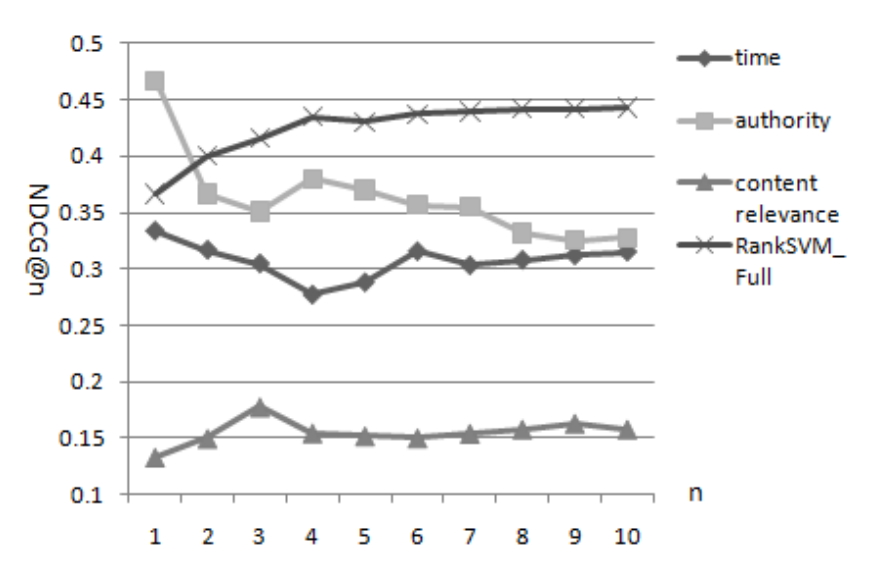
\epsfig{file=img/p2_results.png, width=0.45\textwidth}
\caption{Performance of Four Ranking Methods}
\end{figure}

+ evaluation of the Feature Selection: which are the best features?

+ Combined set of features with best results: URL, Sum\_mention, First\_List, Length, and Important\_follower

+ tested with leave out one, results in figure 3

+ URL is best feature, other features on its own are not significant

\begin{figure}[h]
\centering
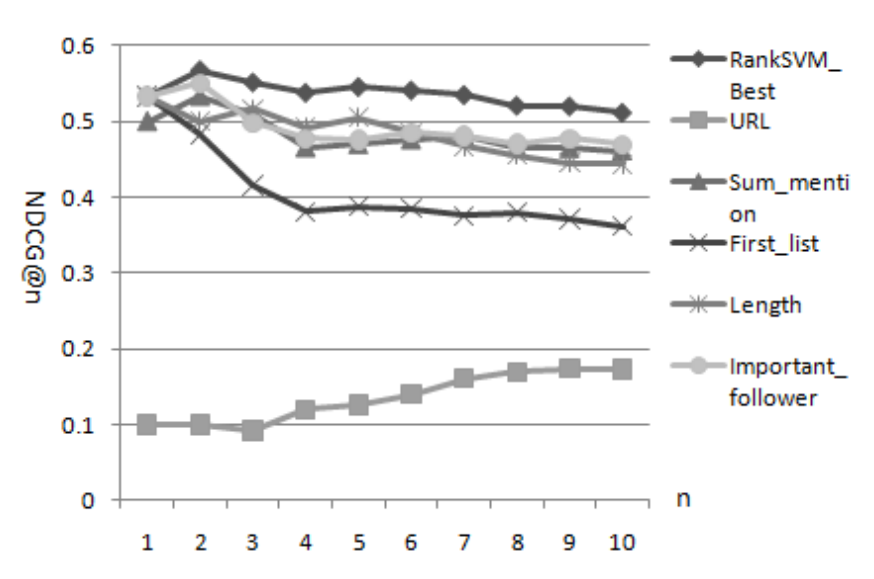
\epsfig{file=img/p2_results_features.png, width=0.45\textwidth}
\caption{Importance of Each Feature}
\end{figure}

% =========================
% =========================
% =========================

%\section{Related Work}

% =========================
% =========================
% =========================

\section{Conclusion}



\bibliographystyle{abbrv}
\bibliography{bibliography} 

\balancecolumns

\end{document}
